\documentclass[12pt,a4paper]{article}%
\usepackage[]{graphicx}\usepackage[]{color}
%% maxwidth is the original width if it is less than linewidth
%% otherwise use linewidth (to make sure the graphics do not exceed the margin)

%2multibyte Version: 5.50.0.2960 CodePage: 1252
\usepackage{amsfonts}
\usepackage{amssymb}
\usepackage[centertags]{amsmath}
\usepackage{graphicx}%
\usepackage{natbib}
\usepackage{color}
\usepackage[dvipsnames,svgnames*]{xcolor}
\usepackage{array}
\usepackage[hidelinks]{hyperref}
\usepackage[font=small,skip=5pt]{caption}
\usepackage[aboveskip=2pt]{subcaption}
\usepackage{amsmath}
\usepackage[]{algorithm2e}
\usepackage{amsthm}
\usepackage{tikz}
\usetikzlibrary{bayesnet}
\usepackage{url}
\usepackage{wasysym}
\usepackage{ulem}
\usepackage{afterpage}
\usepackage{bbm}
\setcounter{MaxMatrixCols}{30}
\providecommand{\U}[1]{\protect\rule{.1in}{.1in}}
\newtheorem{theorem}{Theorem}
\newtheorem{acknowledgement}[theorem]{Acknowledgement}
\newtheorem{axiom}[theorem]{Axiom}
\newtheorem{case}[theorem]{Case}
\newtheorem{claim}[theorem]{Claim}
\newtheorem{conclusion}[theorem]{Conclusion}
\newtheorem{condition}[theorem]{Condition}
\newtheorem{conjecture}[theorem]{Conjecture}
\newtheorem{corollary}[theorem]{Corollary}
\newtheorem{criterion}[theorem]{Criterion}
\newtheorem{definition}[theorem]{Definition}
\newtheorem{example}[theorem]{Example}
\newtheorem{exercise}[theorem]{Exercise}
\newtheorem{lemma}[theorem]{Lemma}
\newtheorem{notation}[theorem]{Notation}
\newtheorem{problem}[theorem]{Problem}
\newtheorem{proposition}[theorem]{Proposition}
\newtheorem{remark}[theorem]{Remark}
\newtheorem{solution}[theorem]{Solution}
\newtheorem{summary}[theorem]{Summary}
\setlength{\topmargin}{0in}
\setlength{\oddsidemargin}{0.1in}
\setlength{\evensidemargin}{0.1in}
\setlength{\textwidth}{6.5in}
\setlength{\textheight}{8.25in}
\numberwithin{equation}{section}

\begin{document}

\section{Introduction}

Consider a high frequency time series with observed values $y_{1}, \dots, y_{T}$, collectively denoted by $y_{1:T}$, with a forecaster interested in the density forecast of the unknown future value $y_{T+S+h}$, where $S \geq 1$. Assuming that a forecast of $p(y_{T+S+h} | y_{1:T})$ is available, uncertainty in the forecast can be reduced by observating and conditioning on the realisations of $y_{T+1:T+S}$ to produce $p(y_{T+S+h} | y_{T+S})$. 

Many models of interest contain a set of global parameters $\boldsymbol{\theta}$ and observation specific latent variables $x_{1:T}$ such that $x_t$ is assumed to follow a Markovian structure. In this case $y_{T+S+h}$ depends on the latent variables $x_{T+1:T+S+h}$, and the forecast uncertainty in $y_{T+S+h}$ can be reduced by first incorporating information contained in realisations of $y_{T+1:T+S}$ to form the posterior densities of $x_{T+1:T+S+h} | x_{1:T}, \boldsymbol{\theta}, y_{1:T+S}$. With certain restrictions on the model, the additional information can be easily included via filtering techniques such as the Kalman filter, however in many cases these restrictions are unsuitable and a computationally costly re-estimation of posterior densities of parameters and latent states must be undertaken.

One of the most common computational techniques for models with latent states is Markov Chain Monte Carlo (MCMC), which involves iterative sampling from a Markov Chain designed to converge to the true posterior distribution. MCMC can have slow convergence rates and generally does not admit parallel processing so that updating the forecast distribution of $y_{T+S+h} | y_{1:T}$ to $y_{T+S+h} | y_{1:T+S}$ after observation of $y_{T+1}, \dots, y_{T+S}$ may not be available before $y_{T+S+h}$ is observed. In this paper we assume that an MCMC will converging before time period $T + S + h$ will be required to begin, at the latest, by time $T$ and hence $y_{T}$ is the last observation that can be included in the MCMC. 

Increasing the speed of estimation will allow more data up to time $T + S$ to be included in the forecast distribution, and this paper explores the use of Variational Bayes to approximate the posterior distribution of several common time-series models with dependent latent states. The the increase in computation speed and resulting increase in observations included in a forecast is contrasted with the decreased statistical accuracy associated with using an approximation to the posterior distribution. We compare several different functional forms of the approximating distribution that are commonly used in the machine learning literature and explore the use of previous MCMC samples to inform the design of the functional form.

\section{Variational Bayes}

Variational Bayes posits a divergence function between the true posterior distribution $p(\boldsymbol{\theta}, x_{1:T} | y_{1:T}$ and some approximating distribution $q(\boldsymbol{\theta}, x | \boldsymbol{\lambda}$, choosing the parameters $\boldsymbol{\lambda}$ for a given functional form $q$ that minimises the divergence function.

We follow the traditional approach, where the divergence function is the Kullback-Leibler (KL) divergence (Kullback and Leibler, 1951) from $q(\boldsymbol{\theta}, x_{1:T}| \boldsymbol{\lambda})$ to the true posterior $p(\boldsymbol{\theta}, x_{1:T} | y_{1:T})$. The KL divergence is defined by
\begin{equation}
\label{KL-def}
KL[q(\boldsymbol{\theta}, x_{1:T} | \boldsymbol{\lambda})\hspace{.1cm}||\hspace{.1cm}p(\boldsymbol{\theta}, x_{1:T} | y_{1:T})] = \int q(\boldsymbol{\theta}, x_{1:T} | \boldsymbol{\lambda}) \ln \left( \frac{q(\boldsymbol{\theta}, x_{1:T} | \boldsymbol{\lambda})}{p(\boldsymbol{\theta}, x_{1:T} |y_{1:T})}\right) d\boldsymbol{\theta} dx_{1:T}
\end{equation}
and can alternatively be expressed as
\begin{equation}
\label{KL-ELBO}
KL[q(\boldsymbol{\theta}, x_{1:T} | \boldsymbol{\lambda})\hspace{.1cm}||\hspace{.1cm}p(\boldsymbol{\theta}, x_{1:T} | y_{1:T})] = \ln(p(y_{1:T})) - \mathcal{L}(q(\boldsymbol{\theta}, x_{1:T} | \boldsymbol{\lambda}), y_{1:T})
\end{equation}
where $\mathcal{L}(q(\boldsymbol{\theta}, x_{1:T} | \boldsymbol{\lambda}), y_{1:T})$ is referred to as the Evidence Lower Bound (ELBO), as it provides a lower bound on the unknown constant $\ln(p(y_{1:T}))$.  $\mathcal{L}(q(\boldsymbol{\theta}, x_{1:T} | \boldsymbol{\lambda}), y_{1:T})$ is defined by
\begin{equation}
\label{ELBO}
\mathcal{L}(q(\boldsymbol{\theta}, x_{1:T} | \boldsymbol{\lambda}), y_{1:T}) = \int q(\boldsymbol{\theta}, x_{1:T} | \boldsymbol{\lambda}) \ln \left( \frac{p(y_{1:T},\boldsymbol{\theta}, x_{1:T})}{q(\boldsymbol{\theta}, x_{1:T} | \boldsymbol{\lambda})} \right) d\boldsymbol{\theta}dx_{1:T},
\end{equation}
and as $\ln(p(y_{1:T}))$ is constant with respect to $\boldsymbol{\lambda}$, maximising (\ref{ELBO}) with respect to $\boldsymbol{\lambda}$ is equivalent to minimising (\ref{KL-def}). 

Equation (\ref{ELBO}) can be maximised using a gradient ascent approach, where we iteratively apply the following update step until (\ref{ELBO}) converges within some pre-specified tolerance:
\begin{equation}
\label{GradAscent}
\boldsymbol{\lambda}^{(m+1)} = \boldsymbol{\lambda}^{(m)} + \rho^{(m)} \nabla_{\boldsymbol{\lambda}} \mathcal{L}(q(\boldsymbol{\theta}, x_{1:T} | \boldsymbol{\lambda}^{(m)}), y_{1:T}).
\end{equation}
$\nabla_{\boldsymbol{\lambda}}\mathcal{L}(q(\boldsymbol{\theta}, x_{1:T} | \boldsymbol{\lambda}^{(m)}), y_{1:T})$ is the vector of partial derivatives of $\mathcal{L}(q(\boldsymbol{\theta}, x_{1:T} | \boldsymbol{\lambda}^{(m)}), y_{1:T})$ with respect to each element of $\boldsymbol{\lambda}$ evaluated at $\boldsymbol{\lambda}^{(m)}$. This update requires some initial values $\boldsymbol{\lambda}^{(0)}$ and a sequence $\rho^{(m)}, m = 1, 2, \dots$ known as the learning rate. If $\rho^{(m)}$ is chosen to satisfy the following conditions the algorithm is guaranteed to converge to a local maximum (Robbins and Munro, 1951).
\begin{align}
&\sum_{m=1}^{\infty} \rho^{(m)} =  \infty \\
&\sum_{m=1}^{\infty} (\rho^{(m)})^2 <  \infty.
\end{align}

Ranganath, Gerrish and Blei (2014) showed that a Monte Carlo estimate of the derivative of the ELBO can be given by
\begin{equation}
\label{ScoreDeriv}
\nabla_{\boldsymbol{\lambda}}\mathcal{L}(q(\boldsymbol{\theta}, x_{1:T} | \boldsymbol{\lambda}^{(m)}), y_{1:T}) \approx \frac{1}{N}\sum_{i=1}^{N} \nabla_{\boldsymbol{\lambda}} [\ln(q(\boldsymbol{\theta}_i, x_{1:T, i} | \boldsymbol{\lambda}^{(m)}))] \ln \left(\frac{p(y_{1:T}, \boldsymbol{\theta}_i, x_{1:T, i})}{q(\boldsymbol{\theta}_i, x_{1:T, i} | \boldsymbol{\lambda}^{(m)})} \right) 
\end{equation}
where $i = 1, \dots, N$ indicates simulations from $q(\boldsymbol{\theta}, x_{1:T} | \boldsymbol{\lambda}^{(m)})$. 
The terms in the sum in (\ref{ScoreDeriv}) can have large variances, and in practice a large value of $N$ is required to ensure a precise estimate of the gradient of the ELBO is obtained, slowing computation. 

The variance can be reduced by the reparameterisation trick of Kingma and Welling (2014), which introduces parameter free noise variables $\boldsymbol{\epsilon}$ and a differentiable transform $f$ such that
\begin{equation}
\label{Reparam}
\boldsymbol{\theta}, x_{1:T} = f(\boldsymbol{\epsilon}, \boldsymbol{\lambda}).
\end{equation}
Kingma and Welling (2014) show that an $f$ exists to transform $\boldsymbol{\epsilon}$ to any continuous random variable, with examples including a location-scale transform of a standard normal noise variable and an inverse-CDF transform of a uniform noise variable. Transforming the variables using
\begin{equation}
\label{changevar}
\int q(\boldsymbol{\theta}, x_{1:T} | \boldsymbol{\lambda}) g(\boldsymbol{\theta}, x_{1:T})  d\boldsymbol{\theta}dx_{1:T} = \int q(\boldsymbol{\epsilon}) g ( f (\epsilon, \boldsymbol{\lambda})) d\boldsymbol{\epsilon})
\end{equation}
and noting that
\begin{equation}
\label{ReparamDist}
\ln(q(\boldsymbol{\theta}, x_{1:T} | \boldsymbol{\lambda})) = \ln(q(\boldsymbol{\epsilon})) - \ln(|J|),
\end{equation}
where $J$ is the Jacobian Matrix of the transformation $f$, allows (\ref{ELBO}) to be rewritten as
\begin{align}
\label{reparamELBO}
\mathcal{L}(q(\boldsymbol{\theta}, x_{1:T} | \boldsymbol{\lambda}), y_{1:T}) &=  \int  q(\boldsymbol{\epsilon}) \ln \left( \frac{p(y_{1:T}, f (\epsilon, \boldsymbol{\lambda}))}{q( f (\epsilon, \boldsymbol{\lambda}) | \boldsymbol{\lambda})} \right) d\boldsymbol{\epsilon} \nonumber \\
&= \int  q(\boldsymbol{\epsilon}) \big( \ln (p(y_{1:T}, f (\epsilon, \boldsymbol{\lambda})) - \ln(q(\boldsymbol{\epsilon})) + \ln(|J|) \big) d\boldsymbol{\epsilon} \nonumber \\
&= \mathcal{L}(\boldsymbol{\lambda}, y_{1:T}).
\end{align}

The derivative of (\ref{reparamELBO}) can be estimated by
\begin{equation}
\label{ReparamDeriv}
\nabla_{\boldsymbol{\lambda}}\mathcal{L}(\boldsymbol{\lambda}^{(m)}, y_{1:T}) \approx \frac{1}{N}\sum_{i=1}^{N} \nabla_{\boldsymbol{\lambda}} \ln (p(y_{1:T}, f(\boldsymbol{\lambda}^{(m)}, \boldsymbol{\epsilon}_i))) + \nabla_{\boldsymbol{\lambda}}\ln(|J(\boldsymbol{\lambda}^{(m)}, \boldsymbol{\epsilon}_i)|),
\end{equation}
where simulations of $\boldsymbol{\theta}$ and $x_{1:t}$ are replaced by simulations of $\boldsymbol{\epsilon}$ from $q(\boldsymbol{\epsilon})$. The variance of the terms in the sum of this estimator is often orders of magnitude lower than the estimator in (\ref{ScoreDeriv}); often $N = 1$ provides a precise enough estimate of the gradient for fast convergence.

\section{MCMC Informed Variational Bayes}

A key decision in Variational Bayes is the choice of the functional form of the approximating distribution $q$. Much of the literature focuses on a generic form of $q$ that can flexibly be applied to many models. However the time-series nature of our application implies that MCMC samples of $p(\boldsymbol{\theta}, x_{1:T} | y_{1:T})$, which provides useful information for constructing the functional form of $q(\boldsymbol{\theta}, x_{1:T+S} | \boldsymbol{\lambda})$ for use in the approximate predictive density, $q(y_{T+S+h} | y_{1:T+S})$. There are two stages to this construction:
\begin{enumerate}
\item Find a well fitting functional form for $q(\boldsymbol{\theta}, x_{1:T} | \boldsymbol{\lambda})$ using the MCMC results.
\item Extrapolate the form of $q$ used for $x_{1:T}$ to $x_{1:T+S}$.
\end{enumerate}
Treating the MCMC samples as 'data', the functional form of $q(\boldsymbol{\theta}, x_{1:T} | \boldsymbol{\lambda})$ can be approached as a traditional distribution fitting problem. Optimal marginal distributions are selected for each parameter by AIC, while a vine copula modelling approach is adopted for the dependence structure following Tran, Blei and Airoldi (2015). Sklar (1959) proves that any joint probability distribution with $k$ variables can be written as the product of the marginals and a copula function,
\begin{equation}
\label{vc1}
p(\omega_1, \dots, \omega_k) = p(\omega_1) \dots p(\omega_k) c(P(\omega_1), \dots, P(\omega_k))
\end{equation}
where $p(\theta)$ is a pdf, $P(\theta)$ is a cdf, and $c(\cdot)$ is a copula. A vine copula is a structure to factorise this copula, increasing the flexibility given to the modeller, and is defined by a set of trees $\mathcal{V} = \{T_1, \dots, T_{k-1} \}$, where
\begin{enumerate}
\item $T_1$ has $k$ nodes corresponding to the $k$ variables, with $k-1$ edges.
\item $T_t, t = 2, \dots, p-1$ has nodes corresponding to the edges in tree $T_{t-1}$
\item Two nodes in tree $T_t$ are joined by an edge only if the associated edges in $T_{t-1}$ share a node. 
\end{enumerate}
Each edge in the vine corresponds to a bivariate copula conditioned on any variables that are shared between nodes, and the product of each of these $k(k-1)/2$ bivariate copulas forms the complete copula. Figure (\ref{fig:vinecop}) provides an example for a four dimensional $\theta$.
\begin{figure}[h]
\centering
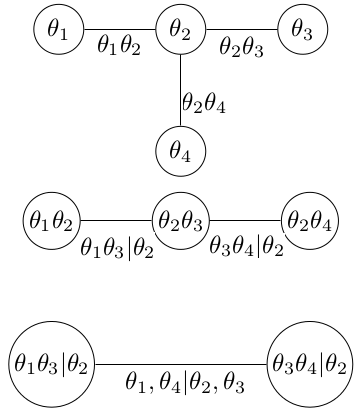
\includegraphics[width=0.4\linewidth,height=\textheight,keepaspectratio]{vines.png}
\vspace{2mm}
\caption{An example of a Vine Copula over four variables. The edges in the top tree represent unconditional bivariate copulas between the parameters on the connected nodes. The second tree edges represent the bivariate copulas for $\theta_1 \theta_3 | \theta_2$ and for $\theta_3 \theta_4 | \theta_2$, the conditioning on $\theta_2$ caused by its appearance in each connected node. The edge in the final tree represents the bivariate copula for $\theta_1, \theta_4 | \theta_2, \theta_3$, as both $\theta_2$ and $\theta_3$ appear in the connected nodes.}
\label{fig:vinecop}
\end{figure}

The Markovian structure of the latent states in the models used provides additional information that can be used in the structure of the vine. Denoting the number of elements in $\boldsymbol{\theta}$ with $k$, allow the first $k$ trees to contain edges that correspond to copulas between different elements of $\boldsymbol{\theta}$, and an element of $\boldsymbol{\theta}$ and $x_t$. The $k+1'th$ tree edges correspond to the copulas $c(x_0, x_1 | \boldsymbol{\theta}, c(x_1, x_2 | \boldsymbol{\theta}), \dots, c(x_{T-1}, x_T | \boldsymbol{\theta}$ and each further tree contains only bivariate copulas between $x_t$ and $x_{t+j}$ conditioned on $x_{t+l}$, where $j > l \geq 1$. Markovian latent states implies that $x_t$ and $x_{t+2}$ are conditionally independent given $x_{t+1}$, so each copula in tree $k+2$ onwards can be set to the independence copula, reducing the number of copula parameters in the vine to be linear in $T$ instead of quadratic. To allow the vine structure to be easily extended to new latent variables $x_{T+1:T+S}$, each $x_t$ node should have edges to the same $\boldsymbol{\theta}$ node. Di{\ss}mann's algorith (Di{\ss}mann, Brechmann, Czado and Kurowicka 2013) can be used to select a well fitting vine structure subject to these restrctions. 

\section{The Dynamic Linear Model}

We begin with the Dynamic Linear Model, which fulfills the neccesary conditions for the Kalman filter to be applicable: (\ref{DLM:Measure}) and (\ref{DLM:Transition}) are linear with Gaussian errors.

\begin{align}
y_t &= \gamma + x_t + \sigma_y \epsilon_t \label{DLM:Measure}\\
x_t &= \phi x_{t-1} + \sigma_x \nu_t \label{DLM:Transition}
\end{align}
where $\epsilon_t$ and $\nu_t$ are independent $\mathcal{N}(0, 1)$ random variables.

We use the priors

\begin{align}
\gamma &\sim \mathcal{N}(\bar{\gamma}, \sigma^2_{\gamma}) \\
\phi &\sim \mathcal{U}(-1, 1) \\
\sigma^2_y &\sim \mathcal{IG}(\mbox{shape = }\alpha_y, \mbox{scale = }\beta_y) \\
\sigma^2_x &\sim \mathcal{IG}(\mbox{shape = }\alpha_x, \mbox{scale = }\beta_x) \\
x_0 &\sim \mathcal{N}(0, \sigma^2_x(1 - \phi^2)^{-1})
\end{align}
where $\mathcal{IG}(\mbox{shape}, \mbox{ scale})$ denotes the inverse of a Gamma (shape, rate) distribution.

We transform $\sigma^2_y$ and $\sigma^2_x$ so that $\boldsymbol{\theta} = \{\gamma, \phi, \ln(\sigma^2_y), \ln(\sigma^2_x) \} \in \mathbb{R}^4$ and consider three different functional forms for the approximating distribution $q(\boldsymbol{\theta}, x_{1:T} | \boldsymbol{\lambda})$:
\begin{enumerate}
\item $q(\boldsymbol{\theta}, x | \boldsymbol{\lambda}) = \mathcal{N}(\boldsymbol{\psi}, \textbf{V})$, where $\textbf{V}$ is a diagonal matrix.
\item $q(\boldsymbol{\theta}, x | \boldsymbol{\lambda}) = \mathcal{N}(\boldsymbol{\psi}, \boldsymbol{\Sigma})$, where $\boldsymbol{\Sigma}$ allows non-zero off-diagonal terms.
\item  $q(\boldsymbol{\theta}, x | \boldsymbol{\lambda}) = \prod \left(q(\theta_i) q(x_{it})\right) c(\boldsymbol{\theta}, x)$ where the form of the copula $c$ and marginals are informed by an out of date MCMC sample.
\end{enumerate}
The first two functional forms are transformation of standard normal noise variables while the third is a transformation of uniform noise variables.

We use three MCMC based approaches for forecasting, listed in increasing computational complexity:
\begin{enumerate}
\item Run the full MCMC to obtain $p(\boldsymbol{\theta}, x_{1:T} | y_{1:T})$ and perform an $S+h$ step ahead forecast of $p(y_{T+S+h} | y_{1:T})$, marginalising out the variables $\boldsymbol{\theta}$ and $x_{1:T}$ using draws from $p(\boldsymbol{\theta}, x_{1:T} | y_{1:T})$.
\item Using the MCMC from approach 1, use the Kalman filter to update the distribution of $x_{T+1:T+S+h}$ after $y_{T+1:T+S}$ is observed to obtain the $h$ step ahead forecast of $p(y_{T+S+h} | y_{1:T+S})$. This method does not condition the posterior distribution of $\boldsymbol{\theta}$ on new observations.
\item Run the full MCMC to obtain $p(\boldsymbol{\theta}, x_{1:T+S} | y_{1:T+S})$ and perform a $h$ step ahead forecast of $p(y_{T+S+h} | y_{1:T+S})$, marginalising out the variables $\boldsymbol{\theta}$ and $x_{1:T+S}$. We assume that the computational time to run this MCMC after observation of $y_{T+S}$ is greater than the time period between $y_{T+S}$ and $y_{T+S+h}$, but this provides a benchmark for comparision with Variational Bayes methods.
\end{enumerate}

We use three similar approaches for VB:
\begin{enumerate}
\item Optimise the distribution $q(\boldsymbol{\theta}, x_{1:T} | \boldsymbol{\lambda})$ after observation of $y_{1:T}$ and perform an $S+h$ step ahead forecast of $q(y_{T+S+h} | y_{1:T})$, marginalising out the variables $\boldsymbol{\theta}$ and $x_{1:T}$, using draws from $q(\boldsymbol{\theta}, x_{1:T} | \boldsymbol{\lambda})$.
\item Using the distribution $q(\boldsymbol{\theta}, x_{1:T} | \boldsymbol{\lambda})$ from approach 1, use the Kalman filter to update the distribution of $x_{T+1:T+S+h}$ after $y_{T+1:T+S}$ is observed to obtain the $h$ step ahead forecast of $q(y_{T+S+h} | y_{1:T+S})$. 
\item Begin with $q(\boldsymbol{\theta}, x_{1:T} | \boldsymbol{\lambda})$ from approach 1, and update to  $q(\boldsymbol{\theta}, x_{1:T+S} | \boldsymbol{\lambda})$ after observation of $y_{T+1:T+S}$. We perform this by holding the elements of $\boldsymbol{\lambda}$ that correspond to the distribution of $x_{1:T}$ fixed, and maximise (\ref{ELBO}) with respect to the elements of $\boldsymbol{\lambda}$ for $\boldsymbol{\theta}$ and $x_{T+1:T+S}$.
\end{enumerate}

Forecast densities of VB and MCMC can be compared by a numeric calculation of the Kullback-Leibler divergence of samples from both $q$ and $p$, and different updating strategies can be compared by the log-score of a held out $y_{T+S+h}$ value. 

With $T = 50, S = 10$ and $h = 1$, data is simulated from the dynamic linear model described by (\ref{DLM:Measure}) and (\ref{DLM:Transition}) with true parameter values of $\mu = 2, \phi = 0.5, \sigma^2_y = 1$ and $\sigma^2_x = 1$, and hyperparameter values of $ \bar{\gamma} = 0, \sigma^2_{\gamma} = 10, \alpha_y = 1, \beta_y = 1, \alpha_x = 1,$ and $\beta_x = 1$. The simulated data values are shown in Figure (\ref{fig:DLMy}), and the resulting forecast distributions are shown in Figure (\ref{fig:DLMpreddens}). The Kullback Leibler divergence from the VB based predictive density $q$ to the MCMC based predictive density $p$ of $y_{T+S+h}$ is calculated in Table (\ref{Tab:KLdiv}).

\begin{figure}[h]
\centering
\includegraphics{yDLM}
\caption{Data $y_{1}, \dots, y_{T+S+h}$ simulated from a dynamic linear model with $T = 50, S = 10$ and $h = 1$. The black component indicates the observations up to time $T$, which are available for use in an MCMC forecast of $y_{T+S+h}$. The red component indicates the observations from time $T+1$ to $T+S$, which cannot be included in an MCMC forecast. The blue component indicates $y_{T+S+h}$.}
\label{fig:DLMy}
\end{figure}

\begin{figure}[h]
\centering
\includegraphics{PredDensDLM}
\caption{The predictive density of $Y_{T+S+h}$ for each forecasting approach using $50,000$ MCMC samples and the first two Variational Bayes functional forms. Both Variational Bayes methods seems to have closely captured the MCMC based density in each approach. \textit{To add: Copulas}}
\label{fig:DLMpreddens}
\end{figure}

\begin{table}
\centering
\begin{tabular}{| l | c c c |}
  \hline
  & $S+h$ step & $h$ step - Filter & $h$ step - MCMC \\
  \hline
  Diagonal & $-9.35 \times 10^{-9}$ & $-1.89 \times 10^{-9}$ & $\boldsymbol{-6.56 \times 10^{-9}} $ \\
  Non-Diagonal & $\boldsymbol{-6.19 \times 10^{-8}}$ & $\boldsymbol{-3.05 \times 10^{-9}}$ &$-3.69 \times 10^{-9} $ \\
  \hline
\end{tabular}
\caption{The Kullback Leibler divergence between densities in Figure (\ref{fig:DLMpreddens}) from $q$ to $p$. Bold indicates the variational approximation with the lowest divergence in each case. The added flexibility in allowing non-zero covariances in the Non-Diagonal functional form appears to improve the fit to the MCMC results in two of the forecasting approaches.}
\label{Tab:KLdiv}
\end{table}





\newpage
\section{Appendix}

\subsection{Variational Approximations for the Dynamic Linear Model}

The joint distribution $p(y_{1:T}, \boldsymbol{\theta}, x_{1:T})$ for the Dynamic Linear Model is given by

\begin{align}
p(y_{1:T}, \boldsymbol{\theta}, x_{1:T}) &= \prod_{t=1}^{T} \bigg( \mathcal{N}(y_t | x_t + \gamma, \sigma^2_y) \mathcal{N}(x_t | \phi x_{t-1}, \sigma^2_x) \bigg) \mathcal{N}(x_0 | 0, \sigma^2_x (1 - \phi^2)^{-1}) \nonumber \\
&\mathcal{N}(\gamma | \bar{\gamma}, \sigma^2_{\gamma}) \mathcal{U}(\phi | -1, 1) \mathcal{IG}(\sigma^2_y | \alpha_y, \beta_y)\mathcal{IG}(\sigma^2_x | \alpha_x, \beta_x) 
\end{align}
with 
\begin{align}
\ln(p(y_{1:T}, \boldsymbol{\theta}, x_{1:T})) &= -(T/2 + \alpha_y + 1) \ln(\sigma_y^2) -(T/2 + \alpha_x + 3/2) \ln(\sigma_x^2) \nonumber \\
&- \frac{\sum_{t=1}^{T}(y_t - \gamma - x_t)^2}{2 \sigma^2_y} - \frac{x_0^2(1 -\phi^2) + \sum_{t=1}^{T}(x_t - \phi x_{t-1})^2}{2 \sigma^2_x} \nonumber \\
&- \frac{(\gamma - \bar{\gamma})^2}{2 \sigma^2_{\gamma}} - \frac{\beta_y}{\sigma^2_y} - \frac{\beta_x}{\sigma^2_x} + c \label{logjoint}. 
\end{align}

We use Kingma and Welling's (2014) reparameterised approach to the variational approximation in all of our applications, with the transforms detailed in Sections 4.1.1 - 4.1.3.

\subsubsection{The Multivariate Normal Approximations}

The distribution $q(\boldsymbol{\theta}, x_{1:T} | \boldsymbol{\lambda})$ for the first two approaches is defined by the following transformation, where $\epsilon_{1}, \dots, \epsilon_{T+5}$ have independent standard normal distributions.
\begin{align}
\sigma^2_y &= \exp(\mu_1 + L_{11} \epsilon_1)  \label{transform1} \\
\sigma^2_x &= \exp(\mu_2 + L_{21} \epsilon_1 + L_{22} \epsilon_2) \label{transform2} \\
\phi &= \mu_3 + L_{31} \epsilon_1 + L_{32} \epsilon_2 + L_{33} \epsilon_3 \label{transform3} \\
\mu &= \mu_4 + L_{41} \epsilon_1 + L_{42} \epsilon_2 + L_{43} \epsilon_3 + L_{44} \epsilon_4 \label{transform4} \\
x_t &= \mu_{t+5} + \sum_{j=1}^{t+5} L_{t+5, j} \epsilon_j \mbox{ for } t = 0, \dots, T \label{transform5} 
\end{align}

The approximation is parameterised by $\boldsymbol{\lambda} = \{ \boldsymbol{\mu}, \textbf{L} \}$ where $\textbf{L}$ is the lower triangular decomposition of the Multivariate Normal variance matrices $\textbf{V}$ and $\boldsymbol{\Sigma}$. In the case where the diagonal matrix $\textbf{V}$ is used, restrict $L_{ij} = 0$ for $i \neq j$.
The log determinant of the Jacobian is given by
\begin{equation}
\label{logdetjac}
\ln(|J|) = \left(\sum_{i = 1}^{i = T+5} \ln(L_{ii}) + \mu_1 + L_{11} \epsilon_1 + \mu_2 + L_{21} \epsilon_1 + L_{22} \epsilon_2\right).  
\end{equation}

Derivatives of (\ref{logjoint}) with respect to $\boldsymbol{\theta}$ and $x_{0:T}$, as well as derivatives of (\ref{transform1}) - (\ref{logdetjac}) with respect to $\boldsymbol{\mu}$ and $\textbf{L}$ are easily obtained for use in estimating the gradient of the ELBO.

\subsubsection{Copula Approximation}

Di{\ss}mann's algorithm was applied to MCMC draws of $\boldsymbol{\theta} = \{ \sigma^2_y, \sigma^2_x, \phi, \gamma \}$ and $x_{0:T}$. The first tree was estimated via:
\begin{enumerate}
\item Map $\boldsymbol{\theta}, x_{0:T}$ to $(0, 1)^{T+5}$ by taking the empirical marginal CDF of each variable.
\item Calculate the absoluate value of Kendall's Tau, $|\tau_{ij}|$ for  $i, j = 1, \dots, T+5$ between each pair.
\item Find the maximum spanning tree by Kruskal's algorithm with edge weights given by $|\tau_{ij}|$, subject to the restrictions that no edge may be selected between two $x_t$ variables and each $x_t$ must have an edge to the same element of $\theta$. This tree forms $T_1$.
\end{enumerate}
The tree $T_1$ that was selected only permitted one vine factorisation for trees $T_2, \dots, T_k$ so a further application of Di{\ss}mann's algorithm was unneccesary. The full vine copula selected is shown in Figure (\ref{fig:dlmvinecop})

\begin{figure}[h]
\centering
\tikz{ %
    \node[latent] (x) {$x_{0:T}$} ; %
    \node[latent, right = of x] (gamma) {$\gamma$} ; %
    \node[latent, right = of gamma] (sigy) {$\sigma^2_y$} ; %
    \node[latent, right = of sigy] (sigx) {$\sigma^2_x$} ; %
    \node[latent, right = of sigx] (phi) {$\phi$} ; %
    \edge [-] {x} {gamma} ; %
    \edge [-] {gamma} {sigy} ; %
    \edge [-] {sigy} {sigx} ; %
    \edge [-] {sigx} {phi} ; %
    
    \node[latent, below = of x] (xgamma) {$x_{0:T}, \gamma$} ; %
    \node[latent, right = of xgamma] (gammasigy) {$\gamma, \sigma^2_y$} ; %
    \node[latent, right = of gammasigy] (sigysigx) {$\sigma^2_y, \sigma^2_x$} ; %
    \node[latent, right = of sigysigx] (sigxphi) {$\sigma^2_x, \phi$} ; %
    \edge [-] {xgamma} {gammasigy} ; %
    \edge [-] {gammasigy} {sigysigx} ; %
    \edge [-] {sigysigx} {sigxphi} ; %
    
    \node[latent, below = of xgamma] (xsigy) {$x_{0:T}, \sigma^2_y | \gamma$} ; %
    \node[latent, right = of xsigy] (gammasigx) {$\gamma, \sigma^2_x | \sigma^2_y$} ; %
    \node[latent, right = of gammasigx] (sigyphi) {$\sigma^2_y, \phi | \sigma^2_x$} ; %
    \edge [-] {xsigy} {gammasigx} ; %
    \edge [-] {gammasigx} {sigyphi} ; %
    
    \node[latent, below = of xsigy] (xsigx) {$x_{0:T}, \sigma^2_x | \sigma^2_y, \gamma$} ; %
    \node[latent, right = of xsigx] (gammaphi) {$\gamma, \phi | \sigma^2_x, \sigma^2_y$} ; %
    \edge [-] {xsigx} {gammaphi} ; %
    
    \node[latent, below = of xsigx] (x1) {$x_1, \phi | \gamma, \sigma^2_x, \sigma^2_y$} ; %
    \node[latent, left = of x1] (x0) {$x_0, \phi | \gamma, \sigma^2_x, \sigma^2_y$} ; %
    \node[latent, right = of x1] (dots) {$\dots$} ; %
    \node[latent, right = of dots] (xT1) {$x_{T-1}, \phi | \gamma, \sigma^2_x, \sigma^2_y$} ; %
    \node[latent, right = of xT1] (xT) {$x_T, \phi | \gamma, \sigma^2_x, \sigma^2_y$} ; %
    \edge [-] {x0} {x1} ; %
    \edge [-] {x1} {dots} ; %
    \edge [-] {dots} {xT1} ; %
    \edge [-] {xT1} {xT} ; %
    
    \node[latent, below = of x1] (x0x1) {$x_0, x_1 | \boldsymbol{\theta}$} ; %
    \node[latent, right = of x0x1] (x1x2) {$x_1, x_2 | \boldsymbol{\theta}$} ; %
    \node[latent, right = of x1x2] (dots2) {$\dots$} ; %
    \node[latent, right = of dots2] (xT1xT) {$x_{T-1}, x_T | \boldsymbol{\theta}$} ; %
    \edge [-] {x0x1} {x1x2} ; %
    \edge [-] {x1x2} {dots2} ; %
    \edge [-] {dots2} {xT1xT} ; %
}
\caption{The vine copula used for the Dynamic Linear Model. Each node containing $x_{0:T}$ denotes $T+1$ individual nodes connected to the same neighbouring node.}
\label{fig:dlmvinecop}
\end{figure}


\subsubsection{Algorithm Details}

Gradient Ascent is performed with the Adam optimiser from Kingma and Ba (2015). Adam uses estimates of the first two moments of the gradient, and is described in Algorithm (\ref{alg:adam}). We use $\alpha = 0.1, \beta_1 = 0.9, \beta_2 = 0.999$ and $\epsilon = 10^{-8}$.

\begin{algorithm}[H]
 \SetKwInOut{Input}{Input}
 \Input{Method to estimate gradients of $f(\lambda), \alpha, \beta_1, \beta_2, \epsilon$}
 \KwResult{Optimal Parameters $\lambda$}
 Set $m_0 = 0$\;
 Set $v_0 = 0$\;
 Set $t = 0$\;
 \While{not converged}{
  $t = t + 1$
  $g_t = \nabla_{\lambda}f(\lambda)$ \;
  $m_t = \beta_1 m_{t-1} + (1-\beta_1) g_t$ \;
  $v_t = \beta_2 v_{t-1} + (1-\beta_2) v_t$ \;
  $\hat{m}_t = m_t / (1 - \beta_1^t)$ \;
  $\hat{v}_t = v_t / (1 - \beta_2^t)$ \;
  $\lambda = \lambda + \alpha \cdot \hat{m}_t / (\sqrt{\hat{v}_t} + \epsilon)$
  }
 \caption{Adam Optimiser}
  \label{alg:adam}
\end{algorithm}

Increases in $N$, the number of simulations of the gradient of the ELBO per iteration, should increase the accuracy of the estimate and thus reduce the number of iterations required for convergence at a cost to compuation time per iteration. Figure (\ref{fig:RuntimeELBO}) plots the converged value of the ELBO against algorithm run time for a range of values of $N$. On this basis, we select $N = 5$ for the diagonal approximation and $N = 100$ for the non-diagonal approximation.

\begin{figure}[h]
\centering
\includegraphics{RuntimevELBO}
\caption{Converged ELBO value versus total runtime for a range of values of $N$ and approximation functional forms.}
\label{fig:RuntimeELBO}
\end{figure}

\end{document}